\documentclass{superfri}

\usepackage{amssymb}
\usepackage{float}
\usepackage[position=t,singlelinecheck=off]{subfig}
\usepackage{caption}
% ------------

\bibliographystyle{plain}
\begin{document}

%\classify{MSC?}
\author{I.M.~Scientist\footnote{\label{susu}South Ural State University} \and U.R.~Author\footnoteref{susu}}

\title{Predicting I/O-performance in HPC using Artificial Neural Networks}

\maketitle{}

\begin{abstract} %Zusammenfassung
	
The prediction of file access times is an important part for the modeling of the storage systems of super computers. These models can be used to develop analysis tools which support the integration of efficient I/O-behavior.\\
We analyzed the parallel storage system of a super computer by measuring file access times in various test series. Afterwards, different models were developed and tested in their ability of predicting access times. Thereby, models utilizing artificial neural networks achieved better results than linear regression models.
A phenomenon in the measurements of file accesses stands out in particular:
File accesses with equal parameter values have several typical access times.
The steps in the magnitude between these typical access times can be explained with a different processing of the file accesses in the storage system.\\
We developed a method to quantify the significance of knowledge about the internal processing for the prediction of file access times and it proved to be essential.

\keywords{file systems, performance, predicting file access times, artificial neural networks}
\end{abstract}

% -----------------------------------------------------------------------
\section*{Introduction} %Problemdarlegung
\label{sec:intro}

Tools are demanded that help users of HPC-facilities to implement efficient input/output (I/O) in their programs.
It is difficult to find the best access parameters and patterns due to complex parallel storage systems.
Currently users have to optimize their programs at great expense to each system individually without much assistance.
To develop tools which support the implementation of efficient I/O a computational model of the storage system is key.\\
For single hard disk systems such a model can be derived analytically \cite{Ruemmler94anintroduction}; however, for the complex storage system of a super computer these models become too difficult to configure \cite{DBLP:conf/npc/ZhangLZJC10}.
Therefore we searched for good predictors of I/O-performance using a machine learning approach with artificial neural networks (ANNs).\\
In our analysis we used ANNs with different input information for the prediction of access times.
Because of the strong correlation between access time and access size the problem seems to fit linear models.
Our results, however, show that the relation of file access parameters to access time is not sufficiently represented by linear models.
ANNs achieve significantly better results than linear models.\\
The processing of file accesses in a storage system can be viewed as a task that is sequentially propagated along a I/O-path in the storage system.
Starting at the invoking processor the storage system is searching for the data going further and further through the storage hierarchy until all data is found, so it can be returned to the processor.
Our analysis suggests that the I/O-path used by the storage system significantly influences the file access time.
Therefore it becomes key for a good model of access times to derive knowledge about I/O-paths.
Unfortunately I/O-paths are difficult to deal with, as it is unknown which path was used for a file access.

\section{Related work}
\label{sec:related}

Generally storage systems are modeled in two different ways for access time prediction: With white-box- or black-box-modeling \cite{Crume:2013:FML:2538542.2538561}.
\begin{itemize}
	\item \textbf{White-box-modeling}: The storage system itself is simulated. Details of hardware components like rotation speed of the magnetic disk in a hard drive are considered. The processing of a file access can be simulated in the model and the resulting access time is then used as prediction for the actual system.
	Processing and resulting performance can be analyzed in detail on the model.
	\item \textbf{Black-box-modeling}: The model abstracts from the real storage system. 
	System performance is imitated without consideration of its occurrence. %Zustandekommen
	This procedure can also be called emulating.
	In contrast to the white-box-model processing of file accesses can't be analyzed on the model itself.
\end{itemize}
The two ways of modeling are fundamentally different and have to be differentiated.

\subsection{White-box-modeling versus black-box-modeling}
For the in-depth analysis of reasoning for behavior of a storage system a white-box-model is desirable.
On the one hand the modeled system is represented in the model and can thus be examined, on the other hand these models can be very precise if modeled correctly \cite{Ruemmler94anintroduction}.
The problems of white-box-modeling are, however, as obvious as its flaws; they have to be modeled individually for every system and modeling becomes quite intricate for single hard drives \cite{Crume:2013:FML:2538542.2538561}.
To approach the complexity of white-box-modeling Ruemmler and Wilkes analyzed the relevance of different hard drive components for the model deviation to save effort for insignificant parts \cite{Ruemmler94anintroduction}.
However, white-box-modeling is usually used for simple systems like a single hard drive. For these hard drives white-box-modeling is already very demanding, hence for the complex parallel storage system of a super computer it's not a feasible approach \cite{DBLP:conf/npc/ZhangLZJC10}.\\

Application of black-box-modeling is easier and more flexible as it's independent from the individual system.
Stochastic approaches coupled with data mining methods are mostly used for black-box-modeling; for example a combination of regression trees support vector regression \cite{Dai:2012:SDP:2477169.2477214}, or selective bagging classification and regression trees \cite{DBLP:conf/npc/ZhangLZJC10}.

\subsection{Prediction of I/O-performance with ANNs}
Computability of ANNs was reasearched by Rojas \cite{Rojas:1996:NNS:235222} and Cybenko \cite{cybenko:mcss} they demonstrated possibility of modeling non linear systems. Cybenko also proved the \textit{universal approximation theorem} which states that feed-forward networks with sufficient complexity exist that can approximate continuous functions on compact subsets of $\mathbb{R}^n$.\\
Crume et al. developed a method using ANNs which exploits periodic patterns in sequences of file access times \cite{Crume:2013:FML:2538542.2538561}.
A Fourier analysis is used to determine the most important frequencies, which are then used as input information of the ANNs.
In a following publication they move away from Fourier analysis, but then use additional sine waves as input for the ANNs \cite{crumelatent}.
This seems to be a promising approach for access time prediction of single hard drives, where the rotational characteristics of the magnetic disk are an essential consideration. It might, however, be difficult to use for more complex systems.

\subsection{I/O-performance prediction in HPC}
Performance analysis in HPC is a important task to examine the system for improvements in usage.
For instance Liu et al. simulated scheduling algorithms for research \cite{liu2011towards}. 
The simulation used DiskSim for prediction of occurring file accesses \cite{Bucy08thedisksim}.\\
Kunkel et al. utilized access time prediction with decision trees for varying parameterizations of ROMIO for access of non-contiguous data \cite{UMLTPTPONI15}. Instead searching for optimal parameters by testing, they were able to find good values through prediction of performance.

\section{Structure of the analysis}
The storage system can be analyzed with series of measurements.
We use synthetic benchmark-tests were many similar measurements follow each other, instead of using arbitrary access parameters for consecutive accesses.
This approach allows for a in-depth analysis of system behavior for different use cases.\\
The file access parameters are:
\begin{itemize}
	\item \textbf{File-ID}: Identifies the invoked file.
	\item \textbf{Access size}: Number of bytes to read or write.
	\item \textbf{OpType}: Type of file access (read or write).
\end{itemize}
Directly measurable or derivable attributes are:
\begin{itemize}
	\item \textbf{Offset}: Distance of file beginning to the starting point of access.
	\item \textbf{Delta-Offset}: Can be calculated for file access $i$ as Offset[$i$] - (Offset[i-1] + access size[i-1]).
	\item \textbf{Access time}: Time in seconds from initiation of the file access to the termination of the process.
\end{itemize}
Knowledge of internal aspects of the system about the current system utilization or about the storage media that have to be addressed is not directly available.

\subsection{Model of the I/O-path}
The internal processing of a file access in the storage system can be viewed using the I/O-path which is the path from the invoking processor to the storage medium that contains the data. Once the data has been found it is passed-through the levels of storage hierarchy to caches.
The resulting access time depends on the depth of this I/O-path because storage media further along the path are increasingly slower.
(\textbf{figure of storage hierarchy?})
While the first levels in storage hierarchy (Caches) are very quick to respond, the main memory is already magnitudes slower; the same applies for the step into the parallel storage system, that is connected via network to the computer nodes.\\
In particular reading file accesses are effected by the depth of the I/O-path, because writing file accesses are usually addressed to the bottom of storage hierarchy to propagate the change to all levels.
As data in the volatile memory is exchanged frequently the I/O-paths to similar file accesses can change with time.

\subsubsection{I/O-path for access time prediction}
Due to the exponential decay of processing speed in the hierarchy, file accesses with similar access parameters, but varying I/O-path, are differentiated with a step in the magnitude of access time.
As the access time is dominated by the slowest component along the I/O-path, a step in the measured access time occurs between to I/O-paths of diverging length.
In figure \ref{fig:io_paths} measurements of reading file accesses can seen, this figure will be discussed in further detail in the following chapter.
\begin{figure}
	\centering
	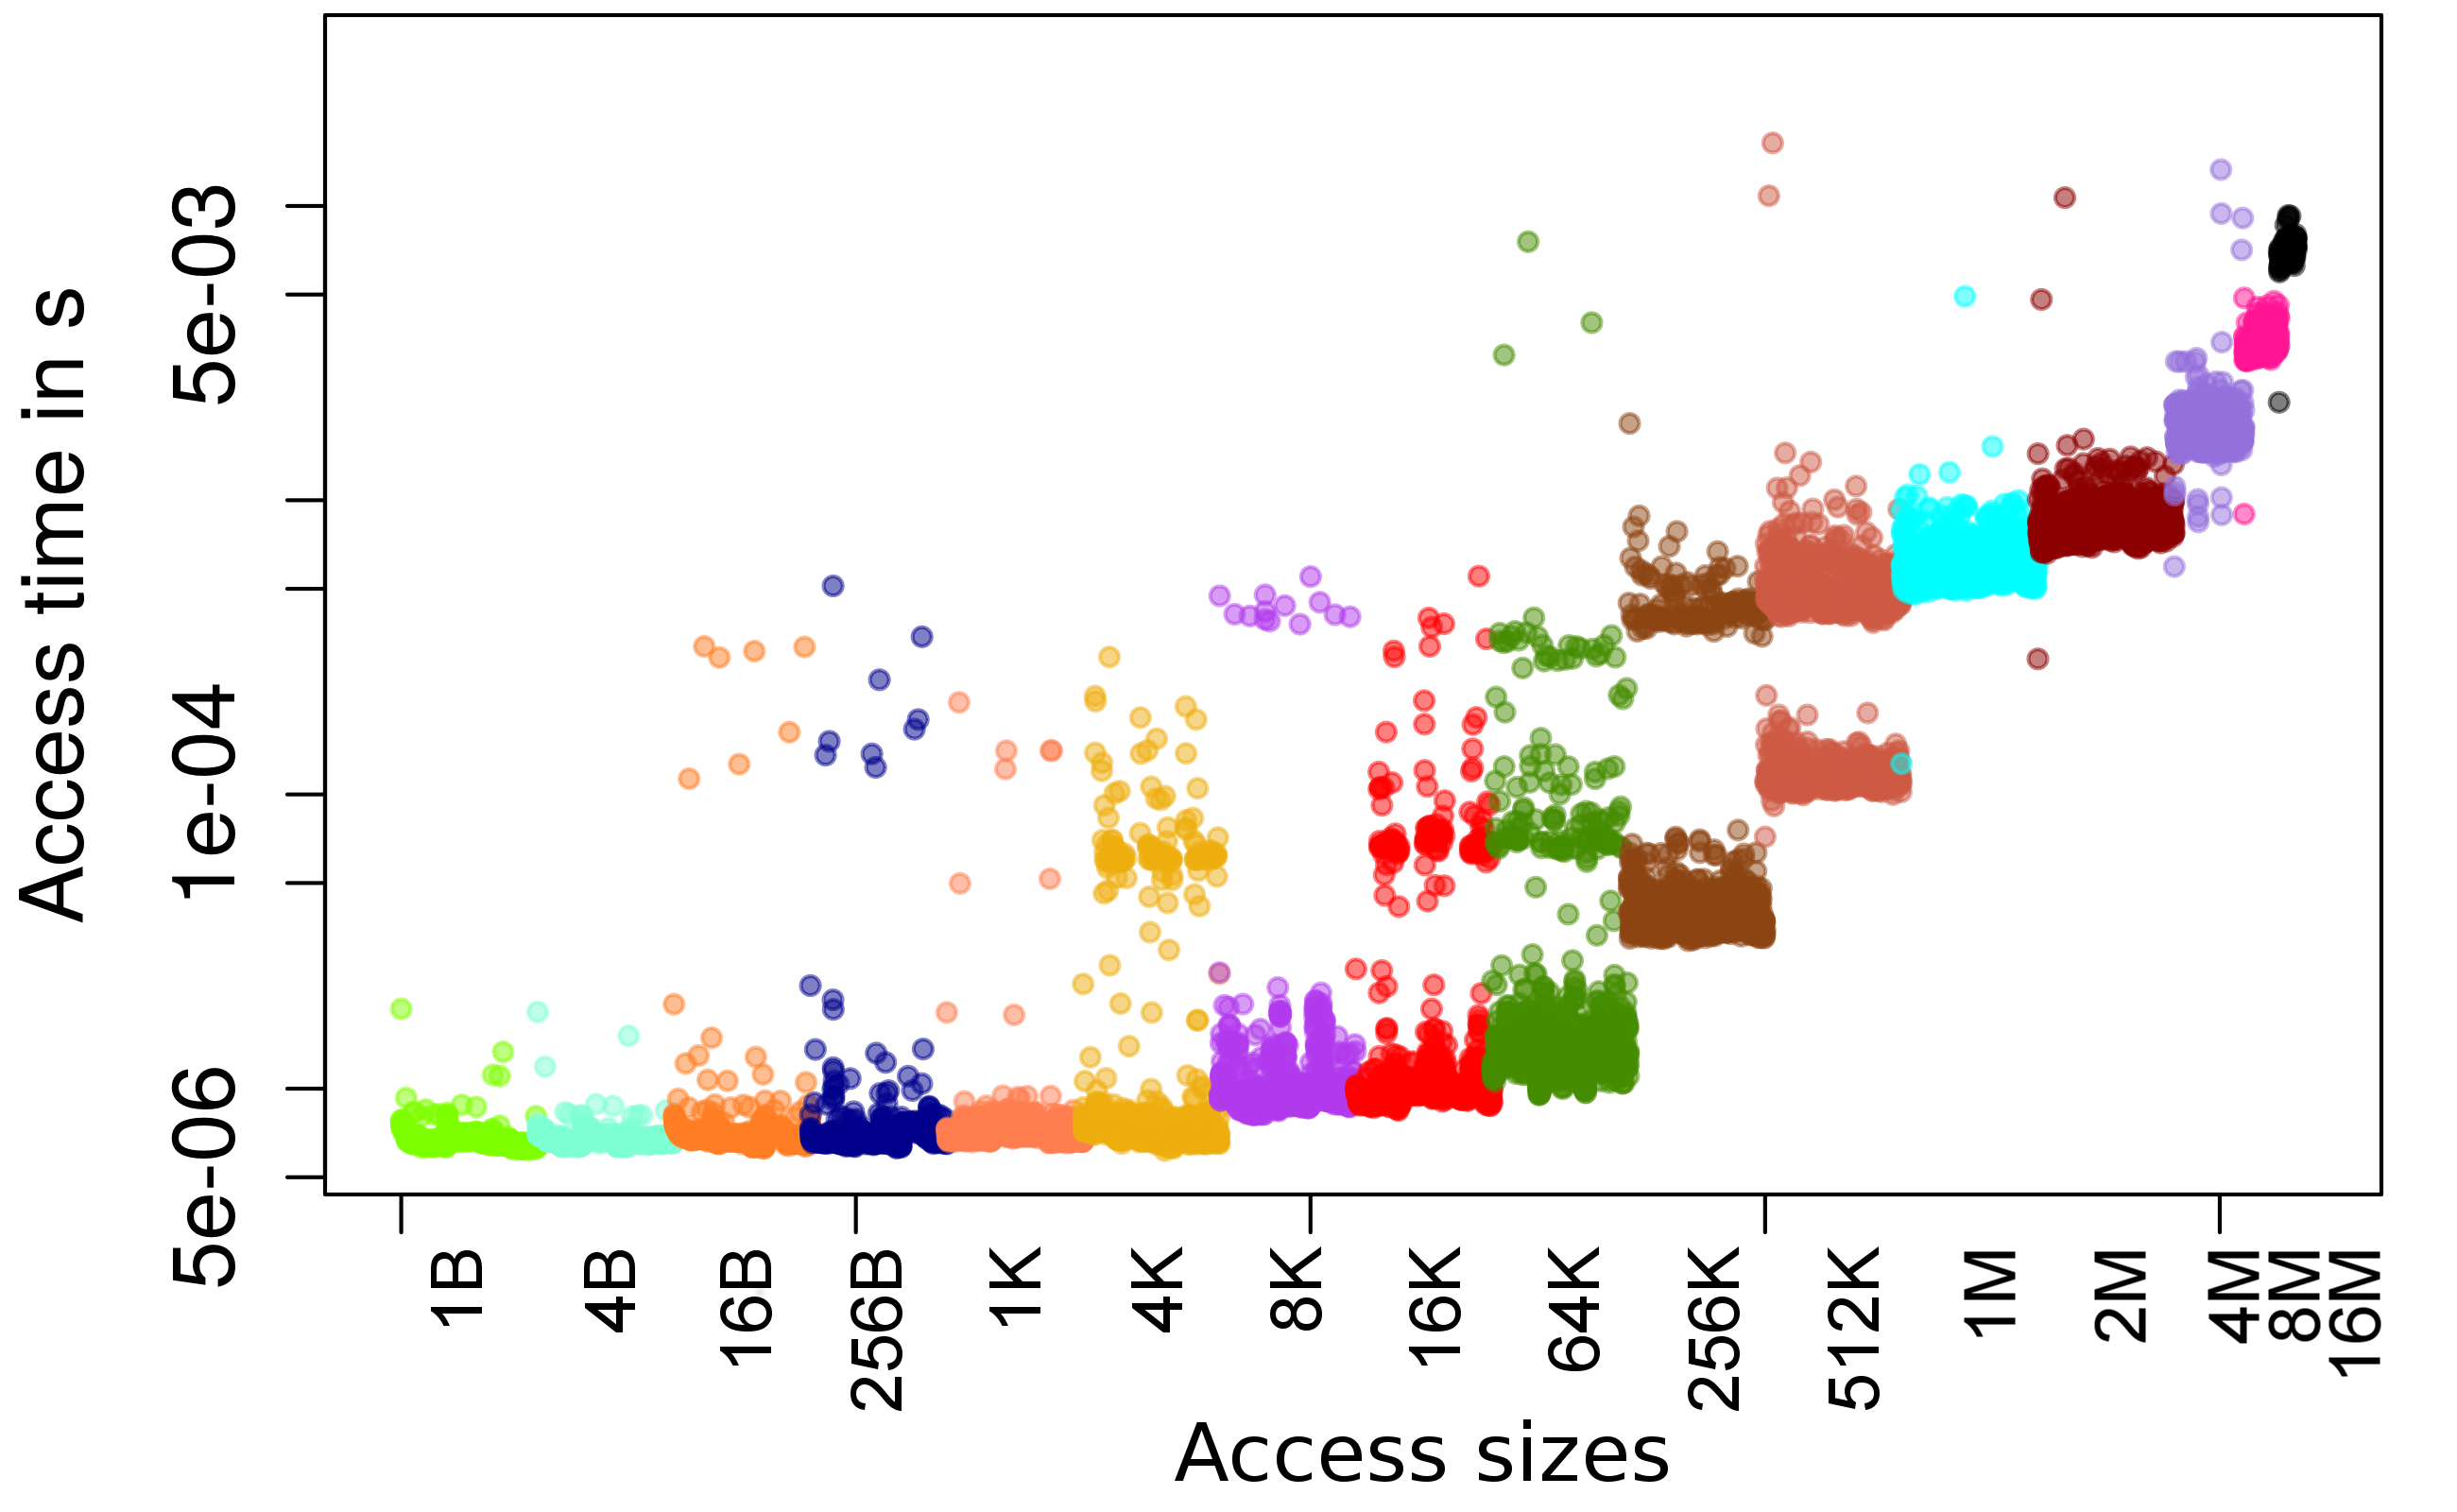
\includegraphics[width=.47\textwidth]{src/plot_SizeSorted_log_read_seq.png}
	\caption{Measurements of reading file accesses. Access sizes increase from left to right and all measurements with equal access parameter values have the same color.}
	\label{fig:io_paths}
\end{figure} 
The different groups of measurements with equal access parameter values (points with the same color) are clearly visible.
Like described previously the different groups are differentiated with a step in the magnitude of access time and can be explained with varying I/O-paths.

\subsection{Error classes}

\subsection{Models}

\section{Evaluation}

\subsection{Test system}

\subsection{Benchmark-tests}

\subsection{Analysis of measurements}
\label{sec:measurements}

\subsection{Analysis of error classes}

\subsection{Prediction of file accesses}

\section{Conclusion and future work}


\ack{Put the acknowledgements after the last section, like this.}
\openaccess

\bibliography{literatur}

%\received{September 25, 2013}

\end{document}
